\documentclass{article}
\usepackage{amsmath}
\usepackage{graphicx}
\usepackage{tikz}

\begin{document}

\begin{center}
    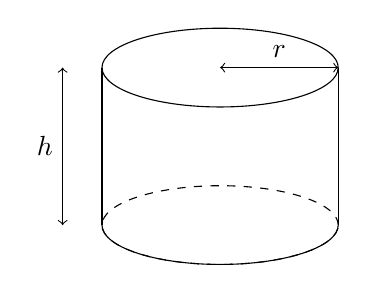
\begin{tikzpicture}
        % Draw the cylinder
        \draw[dashed] (0,0) ellipse (1.5 and 0.5);  % bottom ellipse
        \draw (0,2) ellipse (1.5 and 0.5);  % top ellipse
        \draw (-1.5,0) -- (-1.5,2);  % left side
        \draw (1.5,0) -- (1.5,2);  % right side
        \draw (-1.5,0) arc[start angle=-180,end angle=0,x radius=1.5,y radius=0.5];  % bottom solid line
        
        % Draw the radius from the center of the top ellipse
        \draw[<->] (0,2) -- (1.5,2) node[midway,above] {$r$};  % radius

        % Draw height label
        \draw[<->] (-2,0) -- (-2,2) node[midway,left] {$h$};  % height
    \end{tikzpicture}

    \hspace{2cm}  % Spacing between diagram and equations

    \begin{minipage}{3cm}
        \[
        A = 2\pi r h
        \]
        \[
        V = \pi r^2 h
        \]
    \end{minipage}

    \vspace{1cm}

    \textbf{Cylinder}
\end{center}

\end{document}
